\subsection{Simulations of Membrane Permeation by 1-Butanol}

\subsubsection{Introduction}
The ability of a drug-like molecule to cross (or permeate) a lipid bilayer has been of great interest to drug discovery \citep{zhang_mechanistic_2022}, but is challenging to simulate due to the long timescales involved. 
In this tutorial, we will use WESTPA 2.0 to simulate pathways for membrane permeation by a small molecule (1-butanol) and calculate the permeability coefficient. 
Our WE protocol employs and explains two new features in WESTPA 2.0 \citep{russo_westpa_2022}: (i) the Minimal Adaptive Binning (MAB) scheme \citep{torrillo_minimal_2021}, and (ii) the HDF5 framework for efficient restarting, storage, and analysis of a WE simulation.

\textbf{Learning Objectives.} This tutorial demonstrates how steady state WE simulations can be used to generate pathways and permeability coefficients for membrane permeation by a small molecule.  
Specific learning objectives include:
\begin{enumerate}
    \item How to set up a double membrane bilayer system for permeability studies;
    \item How to use the highly scalable HDF5 framework for more efficient restarting, storage, and analysis of simulations;
    \item How to apply the minimal adaptive binning (MAB) scheme.
\end{enumerate}

\subsubsection{Prerequisites}
In addition to completing the Basic and Intermediate WESTPA Tutorials \citep{bogetti_suite_2019}, a prerequisite to this advanced tutorial is completion of the above \textbf{Advanced Tutorial 3.1}. 
Also required is a working knowledge of the CHARMM-GUI membrane builder, PACKMOL, OpenEye Scientific’s OEChem and Omega toolkits (for system preparation only), MDTraj analysis suite, and the OpenMM 7.6 dynamics engine (for running WE). 

\textbf{Computational Requirements.} The membrane permeability tutorial simulation runs best using, at minimum, a dual-GPU workstation. 
For this tutorial, simulations were tested with a compute node containing both a Titan X (Pascal) GPU and a GTX 1080 GPU, as well as a 16-core Intel Xeon X5550 CPU running at 2.67 GHz with a total of 100 GB of system memory. 
In the case a user does not have a GPU and only CPUs, switch between OpenMM's GPU and CPU platforms by changing the platform name in line 22 of \verb|memb_prod.py| to \verb|CPU| instead of \verb|CUDA|. 
The complete tutorial simulation run length (37 iterations) required \textasciitilde4 days of continuous wall clock time on both GPUs, as well as \textasciitilde30 GB of hard disk space with the HDF5 framework and MAB options turned on.

This tutorial uses the OpenMM 7.6 dynamics engine \citep{eastman_openmm_2017} and MDTraj 1.9.5 analysis suite ({\url{https://www.mdtraj.org/1.9.5/index.html}}) for progress coordinate calculations. 
Force fields used in this tutorial can be installed via openmmforcefields ({\url{https://github.com/openmm/openmmforcefields}}). 
System setup and equilibration were performed separately using OpenMM. 
In order to run the companion Jupyter notebook, nglview, matplotlib are required for visualization purposes. 
Other dependencies, including NumPy and MDTraj, are installed through WESTPA 2.0 itself.

\textbf{Quick Start for this Tutorial.} Users can run the following command within the \verb|tutorial-3.2/| directory to install all the software dependencies to an existing conda environment:

\begin{verbatim}
  $ conda env update --name <your WESTPA conda env> 
                               --file environment.yml
\end{verbatim}

\subsubsection{Preparing the simulation}
The following preparation steps are already completed and the resulting files are provided so that users can begin WE simulations directly. 
The following explanation serves to orient the reader and instruct the reader on how to prepare similar systems for simualtion with WE.

Our system consists of a 1-palmitoyl-2-oleoyl-sn-glycero-3-phosphatidylcholine (POPC) membrane bilayer. 
The 1-butanol-double POPC membrane bilayer system was prepared by piecing together several smaller molecular systems in the following way.
First, a single POPC membrane bilayer was generated using CHARMM-GUI’s membrane builder with 50 lipids per leaflet and zero salt concentration. 
This membrane was then equilibrated using a single GPU with the OpenMM dynamics engine using the standard CHARMM-GUI procedure. 
The membrane plus the outer aqueous layer to the membrane, once combined, (see \textbf{Figure 4}) was equilibrated for an additional 500 ns.
A 2D representation of 1-butanol was generated from an input SMILES string (CCCCO) using OEChem, and converted to a 3D structure using the Omega TK toolkit. 
The 3D structure of 1-butanol was then solvated with a 2 nm slab of water molecules at a density of 1 gm/cm\textsuperscript{3} using PACKMOL along with the OEChem TK and Omega TK toolkits from OpenEye.
Finally, the full double-membrane bilayer system was assembled by placing the butanol-embedded slab of water at the origin, with a single-membrane system at each z-edge of the water slab. 
The resulting system was then subjected to energy minimization and equilibrated before the initiated WE simulations of butanol permeating the membrane bilayer were initialized. 

\begin{figure}[t]
\centering
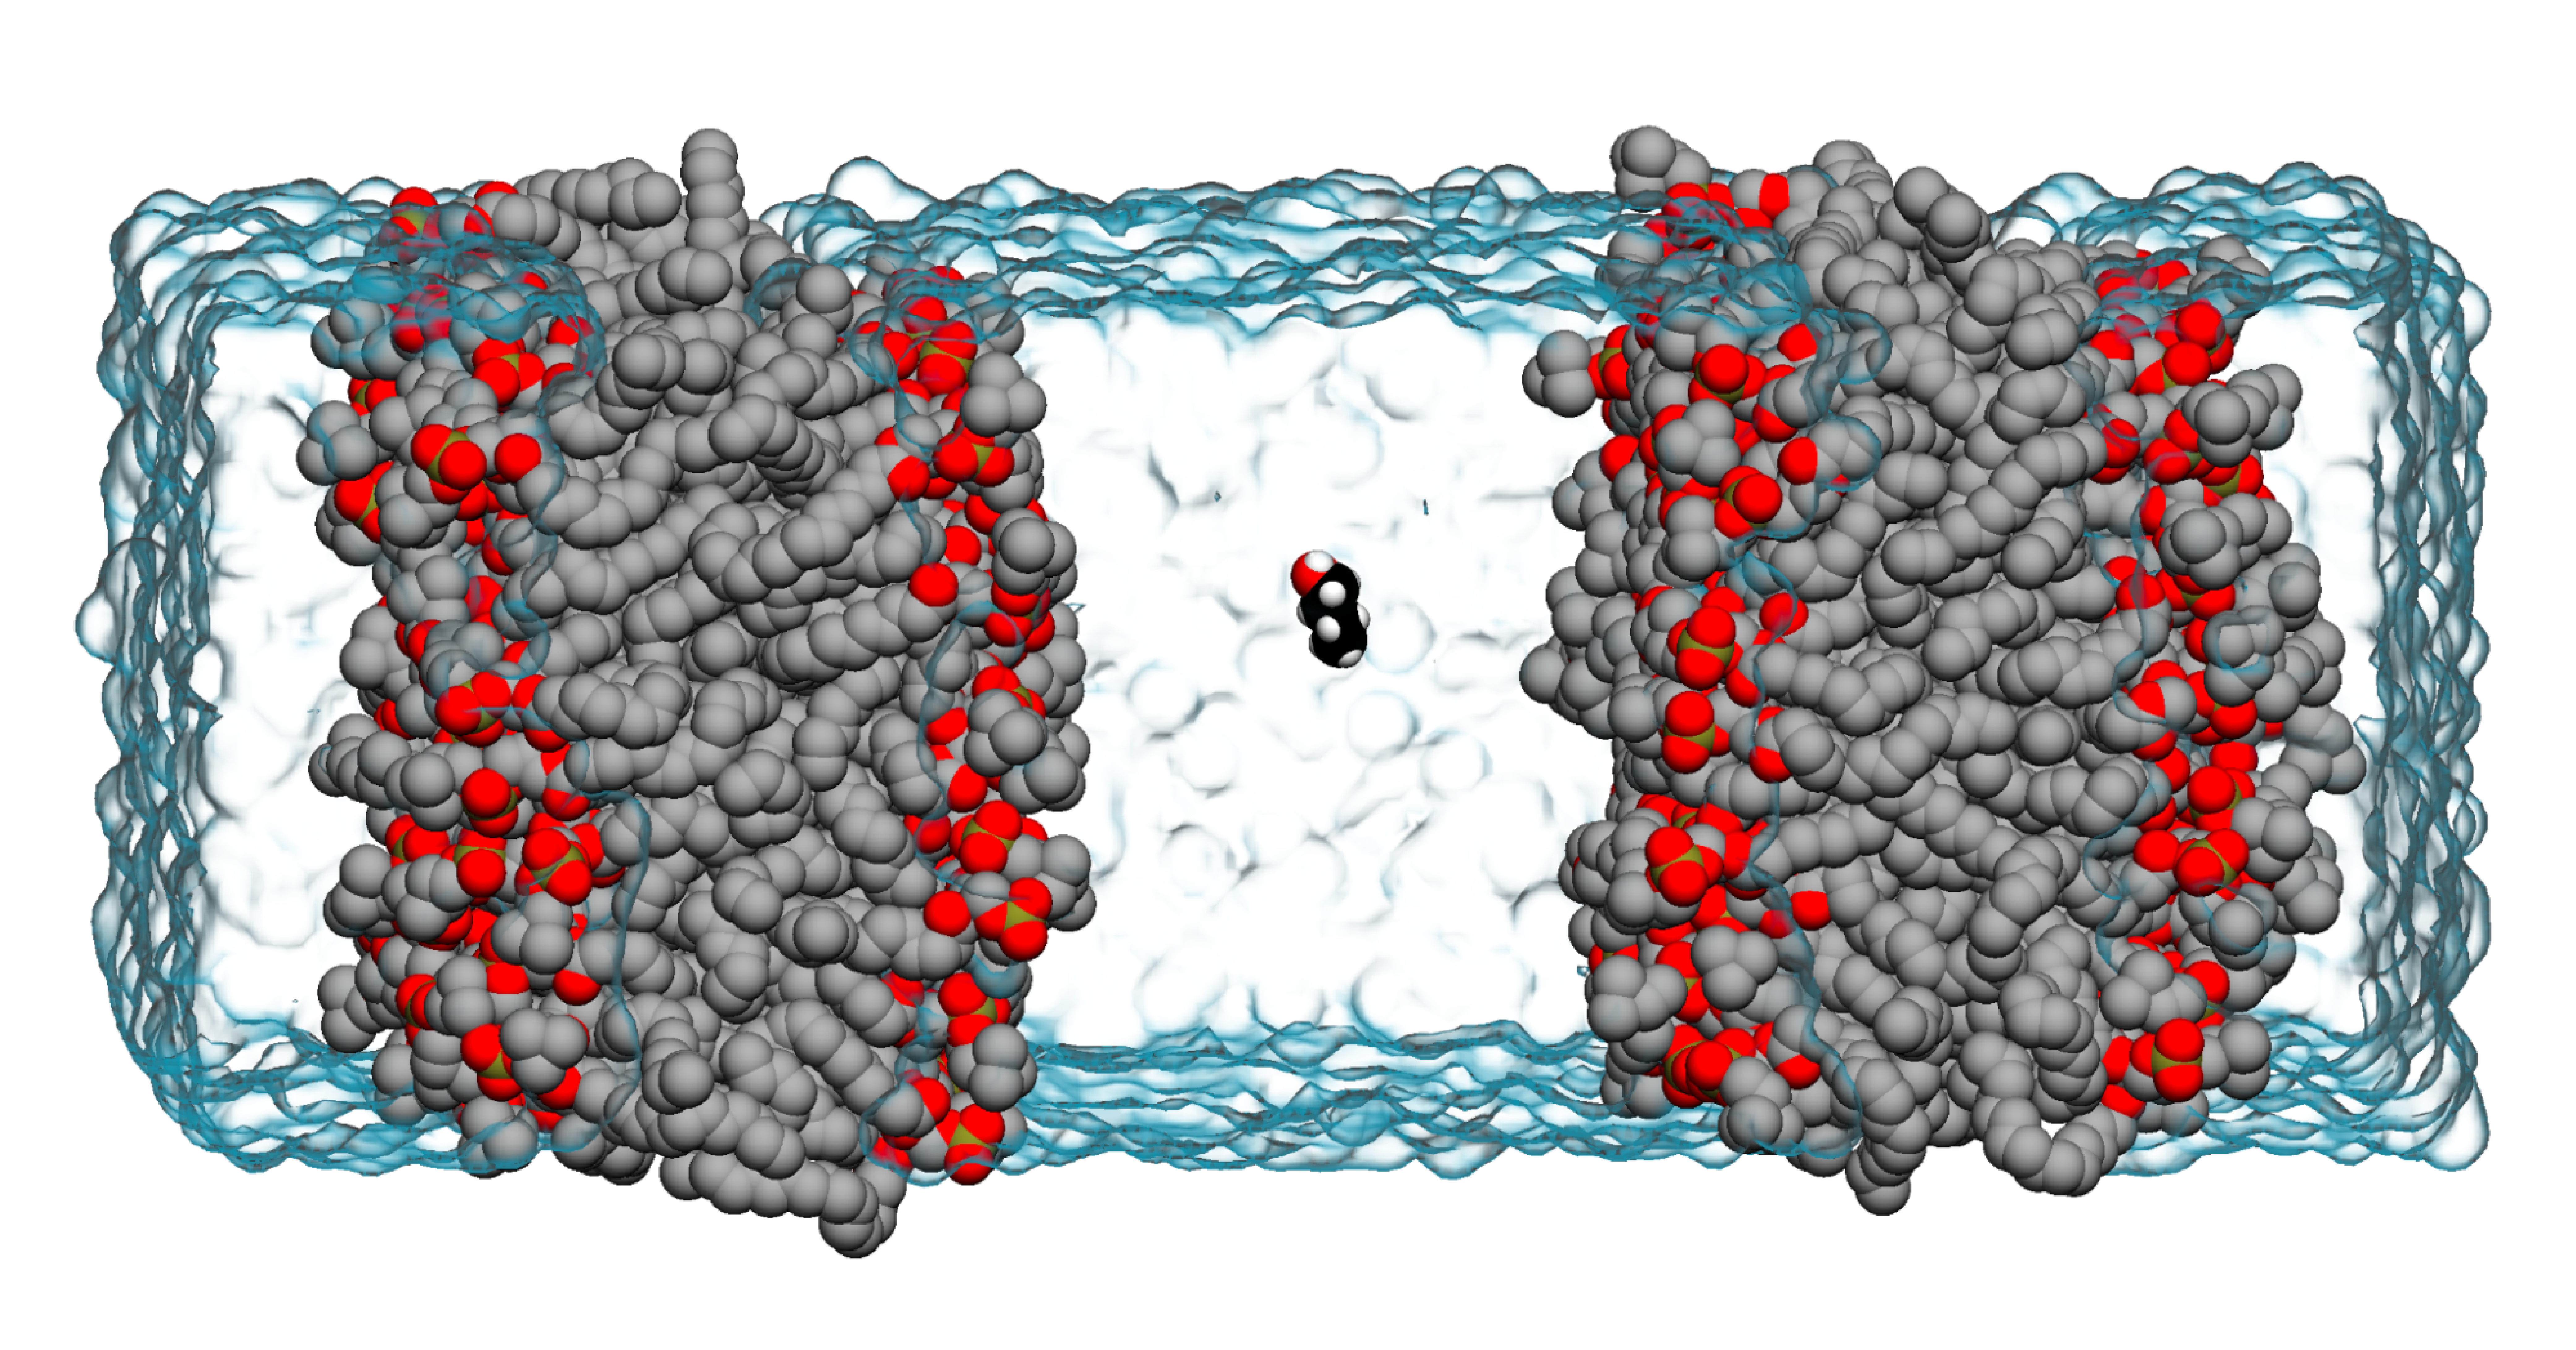
\includegraphics[width=\columnwidth]{figures/Figure4_membrane.pdf}
\caption{The equilibrated double-membrane bilayer system used for initiating WE simulations of membrane permeation by 1-butanol in this tutorial. 
Both the POPC membrane bilayers (gray; hydrogens removed for clarity) and 1-butanol (black) are represented in van der Waals representation, while layers of explicit water molecules are shown as a transparent blue surface.}
\end{figure}

\textbf{The System.} In this tutorial, we will run a WE simulation of 1-butanol crossing one membrane of a double POPC membrane bilayer system. 
To run the WESTPA 2.0 simulation, the AMBER LIPID17 force field is applied to all POPC lipids, explicit water molecules are represented by the TIP3P model, while the parameters for 1-butanol were taken from the GAFF 2.11 force field. 
All force field parameters were applied using the openmmforcefields Python package.

\textbf{Progress Coordinate.} The progress coordinate (z) is defined as the (signed) distance from the center of mass (COM) of the butanol molecule to that of the closest membrane. 
The width of a single leaflet of the membrane is roughly 2 nm, so if z $\leq$ 2 nm, between -2 and 2 nm, or >2 nm indicates that the butanol molecule has not crossed, is crossing, or has crossed the membrane. 
A target state of z $\geq$3.5 nm is used to recycle trajectory walkers. 
The actual computation is performed by measuring the signed distances between the COMs of butanol and each of the two membranes, z\textsubscript{1} and z\textsubscript{2}, using the MDTraj analysis suite and then taking the larger value of the two, z=max(z\textsubscript{1}, z\textsubscript{2}).

\textbf{Preparing the Simulation Environment.}  Once we have constructed and equilibrated the 1-butanol membrane system, we will prepare the WESTPA system environment. 
First, we will analyze the equilibrated double membrane bilayer system to define an initial progress coordinate. 
The progress coordinate, equilibrated coordinate file (e.g. XML file), and \verb|bstates.txt| file describing the initial basis states are placed in the \verb|bstates/| directory. 
Second, we will edit the \verb|west.cfg| file with options for using the MAB scheme and HDF5 framework. 
To initialize the WESTPA 2.0 environment, we will run \verb|./init.sh|. 
This command will source the WESTPA 2.0 environment, construct the \verb|seg_logs/|, \verb|traj_segs/|, and \verb|istates/| directories, and will run the \verb|w_init| command with the correct settings for the target state (z = 3.5 nm) and the basis states constructed above.

\textbf{Adaptive Binning using the MAB Scheme.} By default, this tutorial uses a manual, fixed binning scheme, but can be modified to use the Minimal Adaptive Binning (MAB) module, which adaptively positions bins along the progress coordinate. 
To enable this adaptive binning scheme, uncomment the MAB-related lines in the \verb|west.cfg| file, which specify the \verb|MABBinMapper| as the primary bin mapper type, and comment the lines related to the inner \verb|RectilinearBinMapper|. 
Next, define \verb|n_bins| (the number of MAB bins placed per progress coordinate dimension) in the same section of the \verb|west.cfg| (e.g., if a two-dimensional progress coordinate is being used, \verb|[20, 20]| indicates 20 bins in each dimension). 
It is important to note that if the recycling of trajectories at a target state is desired within the MAB framework, recursive bins must be specified by adding a \verb|MABBinMapper| inside of a \verb|RecursiveBinMapper| outer bin and defining the target state in terms of the recursive outer bins. 
An example of a MAB recursive binning scheme is shown below:

\begin{verbatim}
  # The main WEST configuration file for a simulation.
  ---
  west:
    system:
      system_options:
        bins:
          type: RecursiveBinMapper
          base:
            type: RectilinearBinMapper
            boundaries:
              - [-inf, -44, 34, inf]
            mappers:
            - type: MABBinMapper
              nbins: [20] # Number of bins
              direction: [0] # Split both directions
              skip: [0] # Bin along this dimension
              at: [0]  # Location of MAB mapper
                             relative to base mapper
\end{verbatim}

In the above example, the \verb|at| option in the last line specifies which outer bin to place the MAB scheme inside of range \verb|[-44, 34]|. 
For a two-dimensional progress coordinate, this option will require a list with two values, one for each dimension. 
The \verb|nbins| option specifies the number of MAB linear bins that will be used inside the bin, plus two more bins for extrema and bottleneck trajectories, respectively. 
Optional \verb|direction|, \verb|skip| and \verb|mab_log| parameters can also be specified for the MAB scheme. 
The \verb|direction| parameter (0, -1, or 1) can be used to specify the direction along the progress coordinate for splitting of trajectories, where 0 indicates both directions, -1 indicates the direction of decreasing values along the progress coordinate, and 1 indicates the direction of increasing values along the progress coordinate. 
The \verb|skip| parameter  (1 or 0) designates whether a particular dimension along the progress coordinate will be binned during the simulation, but will be used to define the target state (1 indicates that the dimension will be skipped for binning and 0 indicates that the dimension will not be skipped for binning). 
The \verb|mab_log| parameter, when enabled with \verb|true|, will print MAB-related statistics such as the progress coordinate values of extrema walkers to the \verb|west.log| file. 
Multiple MAB schemes can be added to a recursive binning setup, but only one MAB scheme may be used per each outer bin.

If users choose to combine the application of the MAB scheme with the weighted ensemble steady-state (WESS) plugin \citep{bhatt_steady-state_2010}, which reweights trajectories towards a non-equilibrium steady state, they must provide fixed bins for the reweighting procedure. 
The positions of these fixed bins can be specified in the WESS plugin section of the \verb|west.cfg| file:

\begin{verbatim}
  plugins:
    - plugin: westpa.westext.wess.WESSDriver
      enabled: false
      do_reweighting: true
      window_size: 0.75
      bins:
        type: RectilinearBinMapper
        boundaries:
          - ['-inf', 0.5, 1.0, 1.5, 2.0, 2.5, 'inf']
          
\end{verbatim}

\begin{figure}[t]
\centering
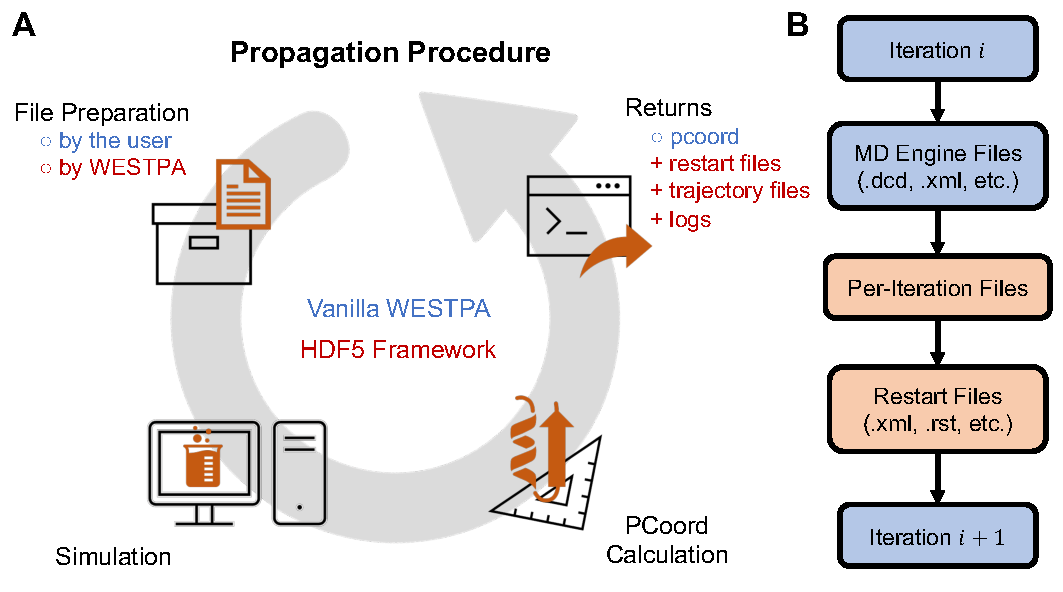
\includegraphics[width=\columnwidth]{figures/Figure5_membrane.pdf}
\caption{Diagrams showing the differences in the propagation procedure between a vanilla WESTPA run and a run with the HDF5 framework. 
A) Procedures for propagating one WE iteration using the original WESTPA 1.0 framework (blue text) and WESTPA 2.0 HDF5 framework (red text). 
Using the WESTPA 2.0 HDF5 framework, the WESTPA software prepares the input files while the user is responsible for returning the progress coordinate (pcoord), restart, trajectory, and optional log files. 
B) Workflow for using the WESTPA 2.0 HDF5 framework. 
Blue: Steps and files from the original WESTPA 1.0 procedure. 
Red: Files generated or prepared by the WESTPA 2.0 HDF5 framework. }
\end{figure}

\textbf{HDF5 Framework.} The setup for a WESTPA simulation with the HDF5 framework is similar to a vanilla one with the addition of the following procedures, which are a more detailed list of the same steps discussed briefly in \textbf{Advanced Tutorial 3.1} above:
\begin{enumerate}
    \item An iteration entry was provided in \verb|west.cfg| under \verb|west.data.data_refs| to specify where and how the per-iteration HDF5 files should be saved and named. 
    \item All the necessary files needed for propagating the next segment, such as state/restart and topology files, are passed on to WESTPA through the environment variable, \verb|$WEST_RESTART_RETURN|, after initialization and propagation of each iteration (\textbf{Figure 5A}). 
    This information is typically placed in the \verb|get_pcoord.sh| and \verb|runseg.sh| files. 
    \item All the trajectory files, and topology files if the topology is not stored as part of the trajectory file, are provided to WESTPA through the environment variable, \verb|$WEST_TRAJECTORY_RETURN|, after the propagation of each iteration. 
    This, again, is typically placed in the \verb|get_pcoord.sh| and \verb|runseg.sh| files. 
    The coordinates of the basis states can be provided through the environment variable during initialization to be stored as the “trajectories” of the zero-th iteration. 
    Note that the procedures described in step 2 and 3 are similar to how the progress coordinates are returned through \verb|$WEST_PCOORD_RETURN| in the vanilla WESTPA simulation. 
    The trajectory and restart files will be saved as part of the per-iteration HDF5 files. 
    In turn, these files do not need to be located and copied over to the directory for propagating the next segment, and they will be automatically extracted and put into the segment folder by WESTPA instead (\textbf{Figure 5B}).
\end{enumerate}

These additional procedures simplify the data management on the user’s end for two reasons. 
First, all the trajectories are stored in a standard way which enables fast and easy access to these trajectories with their associated WE-related data using the newly added analysis module (see Section 3.2.5). 
Second, the restart/state files are much easier to locate as when they are generated than when they are needed in the next iteration, so letting the users pass trajectory and restart files to WESTPA for it to manage frees users from tracking those files themselves which would require the critical knowledge of how two WESTPA-assigned environment variables work (namely, \verb|$WEST_CURRENT_SEG_INITPOINT_TYPE| and \verb|$WEST_PARENT_DATA_REF|). 

For this membrane permeation example, the per-iteration HDF5 files are saved in a folder named \verb|traj_segs/| and named following the pattern \verb|iter_XXXXXX.h5|. 
The basis states are returned to WESTPA in \verb|get_pcoord.sh| as both the “trajectories” of the zero-th iteration and the restart files for propagating the first iteration and recycled walkers. 
The dynamics is propagated using OpenMM for 100 ps for each iteration, and the output trajectory files and state xml files are returned to WESTPA in \verb|runseg.sh|. 
These files are deleted once they are returned in order to save disk space. 
See the sample project setup files for detail.

\subsubsection{Running the WE Simulation}
Similar to other examples, the simulation can be run using \verb|./run.sh| from the top-level permeability tutorial directory.

\subsubsection{Analyzing the WE Simulation}
The analysis of the membrane permeation simulation can be found in the accompanying Jupyter notebook titled Membrane Permeability Tutorial (Analysis). 
In this tutorial notebook, we demonstrate how to extract a complete, continuous pathway of a membrane-crossing event and calculate the incoming flux to the target state from the WE membrane permeation simulation. 
Note that this tutorial assumes that you already have a completed simulation using the HDF5 framework with at least one crossing event (\textasciitilde40 iterations).

\subsubsection{Conclusion}
In this tutorial, we have illustrated the relative ease in which one may use the WESTPA 2.0 software package to perform advanced WE path sampling simulations of membrane permeation for a small molecule (butanol). 
Using a single workstation with commodity GPU hardware, our WE simulation can generate membrane permeation events within a few days of wall-clock time. 
WE simulations, when using the WESTPA 2.0 HDF5 framework and MAB binning scheme, are relatively cost effective, both in terms of total compute time and disk storage.